\documentstyle[11pt,epsfig,fancybox,semcolor,semlayer,doublespace,portrait]
{seminar}
\input clp_utils

\newcommand{\talktitle}[0]{Peter's Question}
\newcommand{\fmttitle}[0]{}
\newcommand{\conftitle}[0]{A Exam}
\newcommand{\myname}[0]{Jim Pivarski}
\newcommand{\affila}[0]{Cornell University}
\newcommand{\talkdate}[0]{October 3, 2002}

\pagestyle{conference}   % From clp_utils.tex

% slide magnification
\slidesmag 1

%%%%%%%%%%%%%%%%%%%%%%%%%%%%%%%%%%%%%%%%%%%%%%%%%%%%%%%%%%%%%%%%%%%%%%%%%%%
% Start document
\begin{document}

% Set page size
\slideheight 7.0in
\slidewidth 8.8in 

% Set array stretch
\renewcommand{\arraystretch}{0.3}
\renewcommand{\slidetopmargin}{0.4in}
\renewcommand{\slidebottommargin}{0.9in}


%%%%%%%%%%%%%%%%%%%%%%%%%%%%%%%%%%%%%%%%%%%%%%%%%%%%%%%%%%%%%%%%%%%%%%%%%%%

% %%%%%%%%%%%%%%%%%%%%%%%%%%%%%%%%%%%%%%%%%%%%%%%%%%%%%%%%%%%%%%%%%%%%%%%%%%%

% \begin{slide*}

% \slideframe{}
% \slideframe*[\dkblue]{Oval}
% \huge
% \heading{Outline}
% \vspace{1 cm}

% \begin{center}
% \begin{minipage}[t]{12 cm}
% \begin{itemize}
% \LARGE \item {\huge Motivation: verify lattice QCD!}
% \LARGE \item {\huge 2 out of 3 Resonances Scanned}
% \LARGE \item {\huge Energy Calibration Systematics}
% \LARGE \item {\huge Other Systematics / Work to be Done}
% \end{itemize}
% \end{minipage}
% \end{center}

% \end{slide*}
 
%%%%%%%%%%%%%%%%%%%%%%%%%%%%%%%%%%%%%%%%%%%%%%%%%%%%%%%%%%%%%%%%%%%%%%%%%%%

\begin{slide*}

\slideframe{}
\slideframe*[\dkblue]{Oval}
\LARGE

\heading{How are Lattice Calculations Done?}

\vfill

\begin{itemize}

  \item Expectation values are expressed as path integrals.
\[ \langle\langle z \rangle\rangle =
   \lim_{T \to \infty} \, 
   \frac{\displaystyle \int {\mathcal D} x(t) \, z(t,x,\dot{x}) \,
   \exp \left(-\int_0^T dt \, {\mathcal L}(t,x,\dot{x})\right)}{\displaystyle
   \int {\mathcal D} x(t) \,
   \exp \left(-\int_0^T dt \, {\mathcal L}(t,x,\dot{x})\right)}
\]

  \vfill

  \item
    \begin{tabular}{p{0.45\linewidth} p{0.45\linewidth}}
      \begin{minipage}{\linewidth}
  	Path integrals can be numerically computed by discretizing time.
      \end{minipage} &
      \begin{minipage}{\linewidth}
  	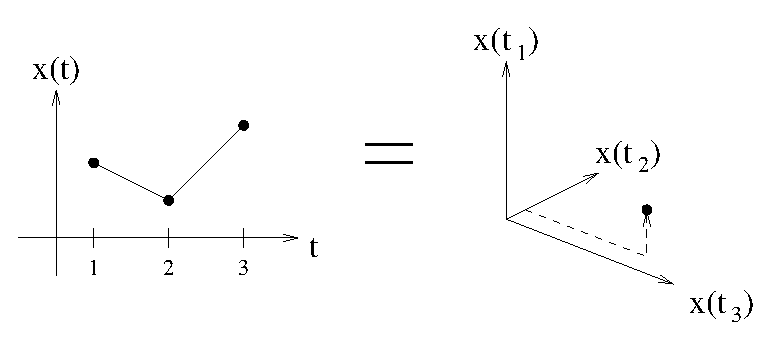
\includegraphics[width=\linewidth]{timesteps.eps}
      \end{minipage}
    \end{tabular}

  \vfill

  \item The number of sample points describing the path is large, so
  the integration space is many-dimensional: integrate with Monte
  Carlo.

  \vfill

  \item For instance, to calculate the ground-state $\psi(x)$,
  randomly generate a set of pairs like this:
\[ \left[ \ f\, ,\, g = \exp\left(-a\sum_{j=0}^{N-1}
             {\mathcal L}\left(ja, x_j, \frac{x_{j+1} - x_j}{
                          a}\right)\right) \ \right] \ a = T/N
\]
  where $f$ is taken uniformly from [$0$,$1$], $x_0 = x_N = x$ and the
  remaining $x_i$ are uniformly distributed in [$-L/2$,$L/2$]. Then
  $\left| \psi(x) \right|^2 e^{-E_0 T} \approx L^{N-1} \,
  \mbox{frac}(f<g)$ for large $T$.

\end{itemize}

\vfill

\end{slide*}

%%%%%%%%%%%%%%%%%%%%%%%%%%%%%%%%%%%%%%%%%%%%%%%%%%%%%%%%%%%%%%%%%%%%%%%%%%%

\begin{slide*}

\slideframe{}
\slideframe*[\dkblue]{Oval}
\LARGE

\begin{minipage}{\linewidth}

\heading{Making the Calculations More Efficient}

\begin{itemize}

  \item Don't use the rejection method to distribute the random
  deviates, but something like the Metropolis algorithm.

  \item Calculate derivatives (and second derivatives) with
  expressions that are correct to higher orders in $a$.

\end{itemize}

\vspace{1cm}

\heading{Doing QCD with Lattice Calculations}

\begin{itemize}

  \item Treat space points as discrete coordinates, like time. Assign
  a real-valued color field $A^a_\mu$ to each space-time point (site).

  \item Formulate a ``link variable''
\[ U_\mu(\vec{x},t) = \exp\left(-i \int_{(\vec{x},t)}^{(\vec{x},t) + a\hat{\mu}}
   g A \cdot dy \right)
\]
  for each link connecting two sites, and re-express the QCD
  Lagrangian in terms of these.

  \item Extrapolate between the sites with perturbation theory.

  \item Tadpole improvement: $\alpha_s(E)$ (running) $\ne$
  $\alpha_{s0}$ (Lagrangian parameter).

\end{itemize}

\end{minipage}

\end{slide*}

% %%%%%%%%%%%%%%%%%%%%%%%%%%%%%%%%%%%%%%%%%%%%%%%%%%%%%%%%%%%%%%%%%%%%%%%%%%%

\begin{slide*}

\slideframe{}
\slideframe*[\dkblue]{Oval}
\LARGE

\begin{minipage}{\linewidth}

\heading{Handling Heavy Quarks: NRQCD}

\vfill

\begin{itemize}

  \item Heavy quark wavefunctions oscillate too rapidly in $t$ to
  efficiently simulate with small lattice spacings.

  \vfill

  \item Lattice spacing is chosen to be ${\mathcal O}(1/m_q)$ to
  exclude relativistic states, heavy quarks are put in by hand as
  wavefunctions with a time-dependence of $e^{-i m_q t/\hbar}$.

\end{itemize}

\vspace{1cm}

\heading{How is $\Gamma_{ee}$ Calculated?}

\vfill

\begin{itemize}

  \item Extract $\left| \psi(0) \right|^2$ from the simulation results.
\[ \Gamma_{ee} = \frac{16 \pi \mbox{$\alpha_{\mbox{\scriptsize E{\tiny \&}M}}$}^2}{
   3 \mbox{$M_\Upsilon$}^2} \left| \psi(0) \right|^2
  \hspace{5mm} \mbox{ and } \hspace{5mm}
  \psi(0) = \left\langle n \, \bigg| \, \mbox{loc} \right\rangle_{\mbox{$^3S_1$}\,z}
\]
  where $\big\langle n \big|$ is the quantum state of a $\Upsilon(nS)$
  polarized in the $z$ direction and $\big| \mbox{loc}
  \big\rangle_{\mbox{$^3S_1$}\,z}$ is the state created by a
  convolution that derives a meson propagator from quark propagators.

\end{itemize}

\end{minipage}

\end{slide*}

% %%%%%%%%%%%%%%%%%%%%%%%%%%%%%%%%%%%%%%%%%%%%%%%%%%%%%%%%%%%%%%%%%%%%%%%%%%%

\begin{slide*}

\slideframe{}
\slideframe*[\dkblue]{Oval}
\LARGE

\begin{minipage}{\linewidth}

\vspace{1cm}

\heading{Handling Systematic Errors in $\Gamma_{ee}$}

\begin{itemize}

  \item Lattice spacing errors: $\left| \psi(0) \right|^2$ scales as $1/a^3$.
  \begin{itemize}

    \item With $1/a$ = 2.4 GeV, uncertainty in $\left| \psi(0)
    \right|^2$ is 13\%.

    \item Need to extrapolate to zero lattice spacing.

  \end{itemize}

  \vfill

  \item Quenched Approximation: $\Gamma_{ee}(2S) / \Gamma_{ee}(1S)$ is
  wrong by a factor of two.
  \begin{itemize}

    \item Include the following two topologies:

    \vfill

    \begin{center}
      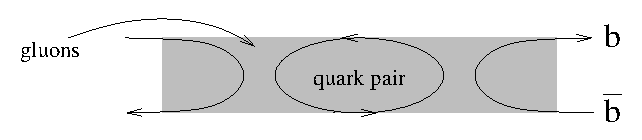
\includegraphics{unquenched2.eps} \\
      \vfill
      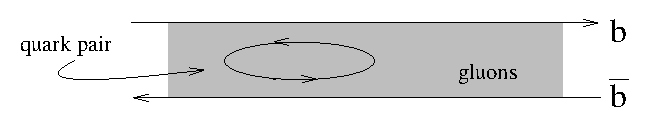
\includegraphics{unquenched1.eps}
    \end{center}

  \end{itemize}

  \vfill

  \item Relativistic corrections: only 5 MeV systematic for the
  $\Upsilon$ masses.

\end{itemize}

\vfill

\end{minipage}

\end{slide*}

% %%%%%%%%%%%%%%%%%%%%%%%%%%%%%%%%%%%%%%%%%%%%%%%%%%%%%%%%%%%%%%%%%%%%%%%%%%%

\begin{slide*}

\slideframe{}
\slideframe*[\dkblue]{Oval}
\LARGE

\heading{Handling Systematic Errors in $\Gamma_{ee}$}

\vfill

\begin{minipage}{\linewidth}
  Even though $\Upsilon(1S)$ and $\Upsilon(2S)$ are below B\={B}
  threshold, light quark loops make a difference. Here is the latest
  calculation of the $\Gamma_{ee}$ ratio, with no loops (quenched),
  two light flavors ($n_f$ = 2), three light flavors ($n_f$ = 3) and
  two light + one strange flavor ($n_f$ = 2+1).

  \begin{center}
    \includegraphics[width=0.8\linewidth]{strange_quark_matters.eps}
  \end{center}

\end{minipage}

\vfill

\vfill

\end{slide*}

\begin{slide*}

\slideframe{}
\slideframe*[\dkblue]{Oval}
\Large

\begin{minipage}{\linewidth}

\heading{References}

\vfill

\begin{flushleft}

\begin{enumerate}

  \item G.~P.~Lepage, ``Lattice QCD for novices,'' {\it Prepared for
  13th Annual HUGS AT CEBAF (HUGS 98), Newport News, Virginia, 26 May
  - 2 Jun 1998}.

  \item G.~P.~Lepage, ``Redesigning lattice QCD,''
  [arXiv:hep-lat/9607076].

  \item C.~T.~Davies, K.~Hornbostel, A.~Langnau, G.~P.~Lepage,
  A.~Lidsey, J.~Shigemitsu and J.~H.~Sloan, ``Precision Upsilon
  spectroscopy from nonrelativistic lattice QCD,'' Phys.\ Rev.\ D {\bf
  50}, 6963 (1994) [arXiv:hep-lat/9406017].

  \item G.~T.~Bodwin, E.~Braaten and G.~P.~Lepage, ``Rigorous QCD
  analysis of inclusive annihilation and production of heavy
  quarkonium,'' Phys.\ Rev.\ D {\bf 51}, 1125 (1995) [Erratum-ibid.\ D
  {\bf 55}, 5853 (1997)] [arXiv:hep-ph/9407339].

  \item A.~Gray {\it et al.} [HPQCD collaboration], ``The Upsilon
  spectrum from lattice QCD with 2+1 flavors of dynamical quarks,''
  [arXiv:hep-lat/0209022].

  \item A.~S.~Kronfeld, ``Beauty and the beast: What lattice QCD can
  do for B physics,'' [arXiv:hep-ph/9310220].

\end{enumerate}

\end{flushleft}

\end{minipage}

\end{slide*}

% %%%%%%%%%%%%%%%%%%%%%%%%%%%%%%%%%%%%%%%%%%%%%%%%%%%%%%%%%%%%%%%%%%%%%%%%%%%

\end{document}

% %%%%%%%%%%%%%%%%%%%%%%%%%%%%%%%%%%%%%%%%%%%%%%%%%%%%%%%%%%%%%%%%%%%%%%%%%%%

% \begin{slide*}

% \slideframe{}
% \slideframe*[\dkblue]{Oval}
% \LARGE
% \heading{}

% \begin{minipage}[t]{\linewidth}

% \end{minipage}

% \end{slide*}

